\chapter{System Architecture}

The system architecture defines the system components, interrelationships and fundamental concepts to note.

\section{Infrared light}

Infrared light extends from the nominal red edge of the visible spectrum at 700 nanometers (430 THz) to 1 mm (300 GHz) \cite{ir_wiki}. The infrared light to be used for NDVI analysis is between 700 and 1000 nm due to silicon response \cite{ir_wiki}, and is known as near infrared light (NIR).

\begin{figure}[H]
\centering
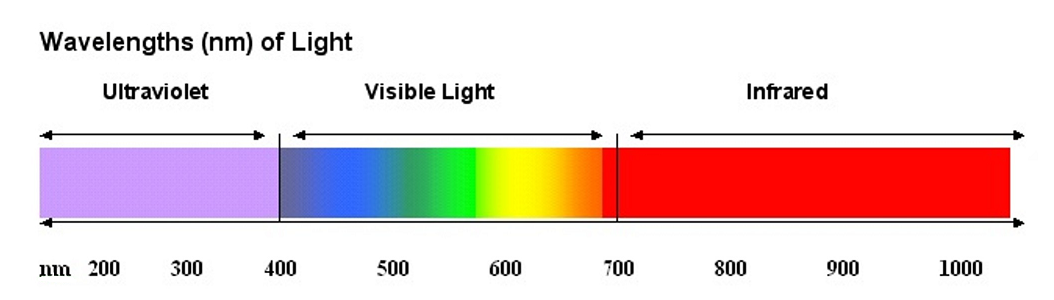
\includegraphics[scale=0.35]{images/ir_spectrum.png}
\caption{Wavelengths of light \cite{ir_spectrum}}
\label{fig:ir_spectrum}
\end{figure}

\section{NDVI}

The normalized difference vegetation index (NDVI) is a simple graphical indicator that can be used to analyze remote sensing measurements, typically but not necessarily from a space platform\footnote{Aerial footage will always be higher resolution, with each pixel capturing $cm^2$ as opposed to $m^2$}, and assess whether the target being observed contains live green vegetation or not\cite{ndvi_wiki} as in Figure \ref{fig:ndvi_british}.

\begin{figure}[H]
\begin{subfigure}{0.5\textwidth}
\centering
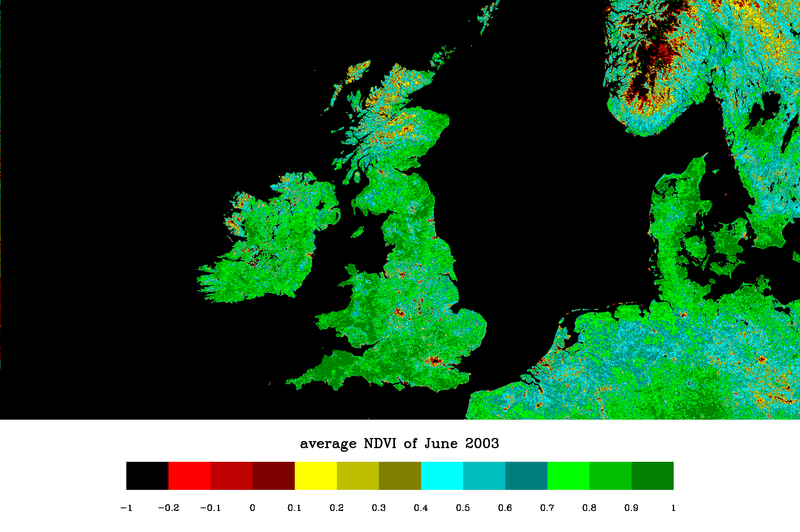
\includegraphics[scale=0.25]{images/NDVI_062003.png}
\caption{June 2003}
\end{subfigure}
\begin{subfigure}{0.5\textwidth}
\centering
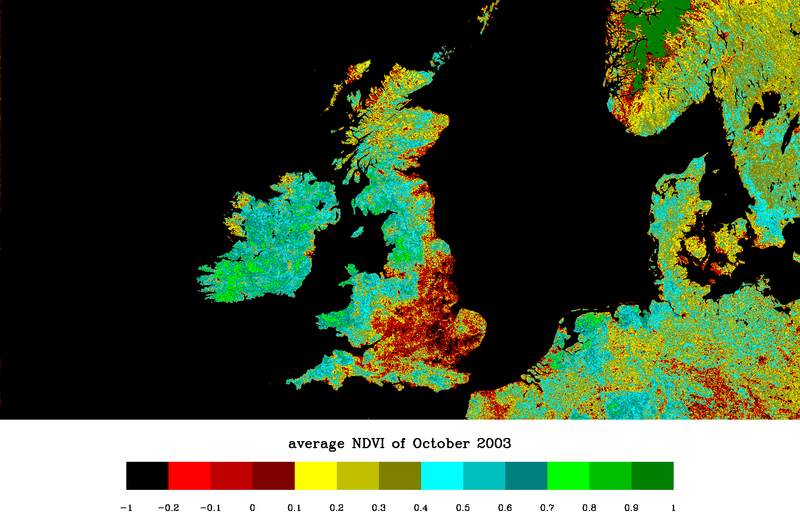
\includegraphics[scale=0.25]{images/NDVI_102003.png}
\caption{October 2003}
\end{subfigure}
\caption{Average NDVI over the British Isles \cite{ndvi_wiki}}
\label{fig:ndvi_british}
\end{figure}

\noindent
The NDVI is calculated using the following formula for each pixel:\\

\begin{equation}\label{eq:ndvi}
{\displaystyle{\mbox{NDVI}}={\frac {({\mbox{NIR}}-{\mbox{Red}})}{({\mbox{NIR}}+{\mbox{Red}})}}}, \in [-1.0, 1.0]
\end{equation}

where red and NIR stand for the spectral reflectance measurements acquired in the red (visible) and near-infrared regions, respectively.

\begin{figure}[H]
\centering
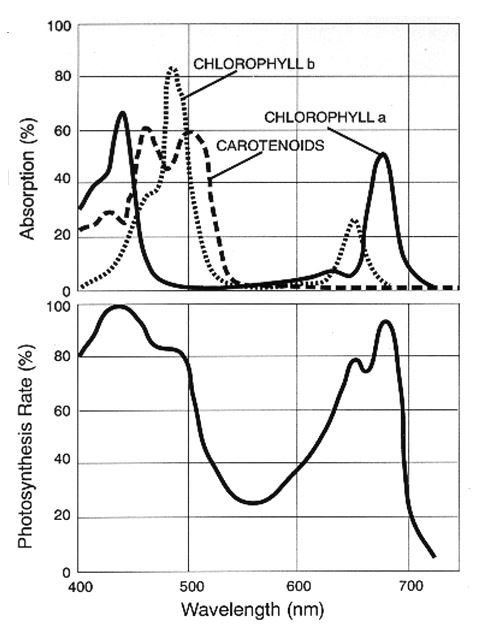
\includegraphics[scale=0.5]{images/chlorophyll.jpg}
\centering
\caption{PAR and absorption spectrum \cite{ndvi_wiki}}
\label{fig:chlorophyll}
\end{figure}

In Figure \ref{fig:chlorophyll}, typical photosynthetic action in the photosynthetically active radiation (PAR) spectral region for live green plants is shown, beside absorption spectra for chlorophyll and carotenoids. Solar radiation is absorbed within this region as a source of energy. \\

Leaf cells re-emit solar radiation in the near-infrared region because the photon energy at wavelengths longer than 700 nm is not large enough to synthesize organic molecules, even though it comprises approximately half of the total incoming solar energy. If it were absorbed, it would only result in damage and overheating of the plant.\\

The NDVI is similar to a mere ratio of infrared light to visible light, yet since it is not normalised, one can have infinite values.\\

The rationale behind the NDVI is that one can exploit the strong differences in plant reflectance to determine their spatial distribution.\\

\section{Hardware Architecture}

\subsection{Filters}

A filter is needed to isolate the NIR channel. If a custom filter is used on a camera with the NIR filter removed, it is possible to isolate a NIR channel without visible light leakage on one or more colour channels. Variants include the Wratten 25A Red Long Pass filter, the Wratten 87 NIR All Pass filter and the Rosco 2008 Blue filter, which allow red and NIR light, only NIR light, and blue and NIR light respectively.\\

The Rosco 2008 Blue filter will be used, for most of the project, as well as the 600nm Dichroic Glass Longpass filter and 500nm Dichroic Glass Bandpass filter from Edmund Scientific, with limited access.

\subsection{Cameras}

Two cameras are required. It is seemingly impossible to capture pure NIR and pure red on separate channels unless the intrinsic bayer matrix (see chapter 4 on intrinsic parameters) is manufactured to allow for it, however, then it would not be cost effective (citation needed).\\

The Sony IMX219 series cameras will be used. They integrate with the Raspberry Pi using a single 15-pin CSI connection.

\subsection{Camera mount}

The cameras will be fixed relative to each other using a PCB substrate so that no rotational or translational drift can occur.

Also, the cameras are to be dampened to prevent a jello-effect due to the rolling shutter cameras. Global shutter cameras are more expensive.

\subsection{On-board processing}

This will be handled by two Raspberry Pis. Both will be used to take photos through each of their single CSI ports. The Raspberry Pis will communicate with each other via direct ethernet connection. Twisted-pair is not necessary since the driver automatically swaps the RX and TX lines.

Initially, one Raspberry Pi was to be used with a camera multiplexer, but it didn't work, and therefore two raspberry pis were used. Just as well, as the flight controller uses all but 1 GPIO pin.

\subsection{Flight controller}

Flight controller is needed to stabilize the airborne vehicle, and set mission waypoints. The Raspberry Pi, Navio2, and camera symbiosis was good since all three together are quite configurable even during flight, compared to other solutions which require hands-on intervention.

\subsection{Drone}

A quadcopter was designed and built to handle all the equipment.

\subsection{Ground Control Station}

An RF linkup (via an ISM band) with a GCS is necessary for pre-flight checks, and monitoring/controlling the status of the vehicle during flight.

\section{Software Architecture}

\subsection{Flight controller}

A real-time kernel will be used for the Ardupilot Firmware used on the flight controller Raspberry Pi.

\subsection{Simultaneous camera triggering}

A few solutions will be investigated, including the use of TCP/UDP packets and 'on the second' triggering.

\subsection{Calibration}

Stereo-calibration using 16x16 square chess board images were used.

\subsection{Stereorectification}

The images were undistorted (see chapter 4 on intrinsic parameters) according to the simultaneous chess board images it was calibrated at.

\subsection{SIFT and NDVI}

Finally, a scale-invariant-feature-transform is applied to the images to align them using an affine transform. An NDVI calculation is applied to the matched images, with a floating point output image. A LUT colourmap is applied to visibly distinguish different areas and their meanings in the final image.

\section{Stiching and Mapping}

A few images are stitched together to show proof-of-concept.